\documentclass{article}
\usepackage[
paperwidth = 12.5cm, 
paperheight=15cm,
textwidth = 12.5cm,
textheight =15cm,
nohead,
nofoot,
nomarginpar,         
margin=0mm]{geometry}
\usepackage{amsmath,amsfonts,amssymb}
\usepackage{tikz,pgfplots}
\usetikzlibrary{arrows,arrows.meta,bending,calc,decorations,shadings,shadows,shapes,shapes.arrows,shapes.geometric}
\usetikzlibrary{calc,fadings,decorations.pathreplacing}
\usepgfplotslibrary{units,fillbetween,groupplots,colorbrewer}
\usetikzlibrary{pgfplots.colorbrewer,}
\usepackage{pgfplotstable}
\usetikzlibrary{3d,spy}
\usepgfmodule{plot}
\usepackage{scalerel}
\usepackage{graphicx}
\usepackage{tikz-dimline}
\usepackage{epstopdf}
\epstopdfsetup{outdir=out/,suffix=-generated}
\definecolor{As}{RGB}{255,255,0}
\definecolor{Al}{RGB}{173,216,230}
\definecolor{Ga}{RGB}{0,128,150}

\definecolor{background}{RGB}{77,77,77}

\definecolor{plane100}{RGB}{0,178,69}
\definecolor{plane010}{RGB}{0,255,208}

\newcommand*{\xMin}{0}%
\newcommand*{\xMax}{14}%
\newcommand*{\yMin}{-7}%
\newcommand*{\yMax}{0}%

\begin{document}
	\thispagestyle{empty}
\begin{tikzpicture}[remember picture,overlay]

%\shade[ball color=magenta, fill opacity=0.0,] (current page.center) circle [radius=1cm] node[scale=3,opacity=0,font=\bfseries](c0) {$\pmb{C_{2v}}$};

%\shade[ball color=cyan, fill opacity=0.8,] ([xshift=-4.3cm]current page.center) circle [radius=2cm] node[scale=7,opacity=1,font=\bfseries](c0) {$C_{2v}$};

\node [draw=blue!60,circle,inner sep=-0.3mm,align=center,ball color=cyan,scale=8](c0) at ([xshift=-4cm]current page.center) {$\displaystyle C_{2v}$};
% \draw ([xshift=5.5cm]c0.east) circle [radius=2cm] node[anchor=center,text width=3.8cm] (c3){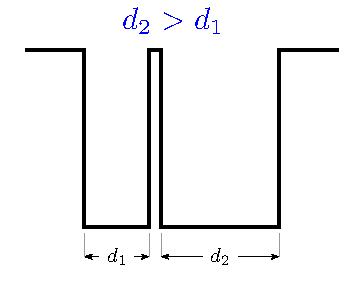
\includegraphics[width=\textwidth]{profiles/c2v-3}};

\node [draw=blue!60,circle,inner sep=0mm,inner sep=-3mm,line width=.5mm](c1) at ([xshift=5cm]c0.east) {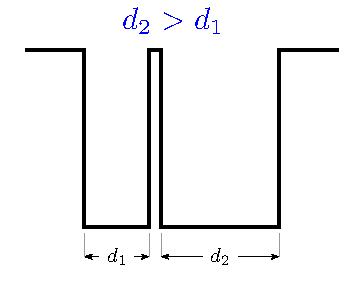
\includegraphics[scale=0.7]{profiles/c2v-3}};
\def\arcccu{235}
\def\arcccd{55}

\draw[color=blue!60,right color=blue,middle
color=blue,fill opacity=0.3,line width=.5mm,draw opacity=1,rounded corners,inner sep=0mm]  
(c0.south east) to [bend left] (c1.south west)  arc (225:140:2.3) -- 
(c1.north west) to [bend left] (c0.north east) arc (45:-45:2.25);


\node [draw=blue!60,circle,inner sep=0mm,inner sep=-3mm,line width=.5mm](c2) at ([xshift=2.5cm,yshift=3.5cm]c0.north east) {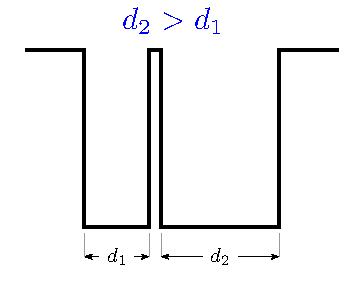
\includegraphics[scale=0.7]{profiles/c2v-3}};

\draw[color=blue!60,right color=blue,middle
color=blue,fill opacity=0.3,line width=.5mm,draw opacity=1,rounded corners,inner sep=0mm]  
(c0.east) to [bend left] (c2.south) arc (270:170:2.3)--
(c2.west) to [bend left] (c0.north) arc (90:0:2.3);

\node [draw=blue!60,circle,inner sep=0mm,inner sep=-3mm,line width=.5mm](c3) at ([xshift=2.5cm,yshift=-3.5cm]c0.south east) {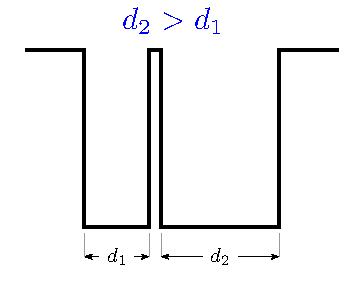
\includegraphics[scale=0.7]{profiles/c2v-3}};


\draw[color=blue!60,right color=blue,middle
color=blue,fill opacity=0.3,line width=.5mm,draw opacity=1,rounded corners,inner sep=0mm]  
(c0.east) to [bend right] (c3.north) arc (90:185:2.3)--
(c3.west) to [bend right] (c0.south) arc (270:360:2.3);
%  ([xshift=6mm,yshift=0mm]c0.south) to [bend left]  ([xshift=-6mm,yshift=0mm]c3.south) 
%  arc (\arcccu:\arcccu-100:1) --
%  ([xshift=-6mm,yshift=16.5mm]c3.south) to [bend left] ([xshift=6mm]c0.north) 
% arc (\arcccd:\arcccd-100:1);

%\node[scale=1.25,blue,xshift=-1mm,font=\bf] at (c3.north west){(f)};









\end{tikzpicture}
	
	


\end{document}